\documentclass[11pt,a4paper]{article}
\usepackage[spanish,es-noshorthands]{babel}
\usepackage{fontspec}
\setmainfont{texgyreheros}[Extension=.otf,UprightFont=*-regular,BoldFont=*-bold,ItalicFont=*-italic,BoldItalicFont=*-bolditalic]
\usepackage[margin=2.2cm]{geometry}
\usepackage{xcolor,graphicx,booktabs,tabularx,longtable,array,enumitem,titlesec,fancyhdr}
\usepackage[most]{tcolorbox}
\usepackage[hidelinks]{hyperref}
\usepackage{xurl}
\definecolor{azul}{HTML}{1C5CAB}
\definecolor{tinta2}{HTML}{52514E}
\definecolor{fondo}{HTML}{F3F7FC}
\titleformat{\section}{\Large\bfseries\color{azul}}{\thesection}{0.6em}{}
\titleformat{\subsection}{\large\bfseries}{\thesubsection}{0.6em}{}
\newtcolorbox{ficha}[1]{enhanced,colback=white,colframe=azul!35,boxrule=0.6pt,arc=2pt,
  title={\bfseries #1},coltitle=azul,colbacktitle=fondo,fonttitle=\normalsize,left=6pt,right=6pt,top=3pt,bottom=3pt}
\newtcolorbox{nota}{colback=fondo,colframe=fondo,arc=2pt,left=8pt,right=8pt}
\setlength{\parskip}{0.5em}\setlength{\parindent}{0pt}
\renewcommand{\arraystretch}{1.2}
\pagestyle{fancy}\fancyhf{}\renewcommand{\headrulewidth}{0pt}
\fancyfoot[L]{\small\color{tinta2}Mérida, Ciudad Esponja · Subtema 1}\fancyfoot[R]{\small\color{tinta2}\thepage}

\begin{document}

{\color{azul}\small\bfseries MÉRIDA CIUDAD ESPONJA}\\[2pt]
{\huge\bfseries Precipitación y eventos de lluvia en Mérida}\\[4pt]
{\large\color{tinta2} Catálogo de fuentes (9 categorías × 3 fuentes), datos y propuesta de visualización}\\[6pt]
{\small\color{tinta2} Subtema 1 · Versión 2 · 1 de octubre de 2026}

\begin{nota}
\textbf{Pregunta del subtema:} ¿Cómo se distribuye la lluvia en Mérida y cómo ha cambiado con el tiempo?\\[3pt]
\textbf{Entregables:} este documento; el Excel \texttt{catalogo\_fuentes\_precipitacion\_merida.xlsx}; y la carpeta
\texttt{datos/}, organizada en una subcarpeta por categoría (\texttt{01\_INEGI} … \texttt{09\_AR}).
\end{nota}

\section{Resumen}

\begin{itemize}[leftmargin=1.2em,itemsep=2pt]
\item \textbf{27 fuentes} en las 9 categorías del proyecto, 3 por categoría. De ellas, 21 ya tienen datos en la carpeta
  (descargados, generados por nosotros o con script y muestra de scraping), 2 solo se pueden consultar en línea
  y 4 están pendientes (3 solicitudes de información y 1 que requiere cuenta de NASA).
\item \textbf{Cuánto llueve:} unos \textbf{1,045 mm al año} en el centro de Mérida (estación 31044, promedio 1991–2020).
\item \textbf{Cuándo llueve:} el \textbf{81\%} cae de mayo a octubre, con picos en junio (184 mm)
  y septiembre (181 mm). Julio baja a 132 mm (canícula).
\item \textbf{Dónde llueve:} más hacia el sur y el oriente, menos hacia la costa. Las isoyetas de INEGI van de 600 mm cerca de Progreso
  a 1,000 mm al sur, y las estaciones del SMN registran 630 mm en Progreso contra 1,000–1,130 mm en Mérida y Conkal.
\item \textbf{Eventos extraordinarios:} 2020 fue el año más lluvioso (1,954 mm en la estación 31097; 1,802 mm en el promedio de Yucatán).
  Cristóbal dejó 215 mm en un día (4-jun-2020). Mérida tuvo declaratorias oficiales por Isidoro (2002), Emily (2005), Dean (2007) y Gamma/Delta (2020).
\item \textbf{¿Qué tan raro es?} Según nuestro ajuste, una lluvia de unos 182–209 mm en 24 h se espera, en promedio, una vez cada 100 años.
  Cristóbal estuvo en ese rango.
\item \textbf{¿Ha cambiado?} El total anual no muestra una tendencia clara (+8.5 mm por década, 1961–2025). Los días con 50 mm o más
  fueron más frecuentes en 2020–2025, pero son pocos años para concluir.
\end{itemize}

\section{Matriz de fuentes: 9 categorías × 3}

{\small
\begin{longtable}{@{}>{\raggedright\arraybackslash}p{2.9cm}>{\raggedright\arraybackslash}p{4.4cm}>{\raggedright\arraybackslash}p{4.4cm}>{\raggedright\arraybackslash}p{4.4cm}@{}}
\toprule
\textbf{Categoría} & \textbf{Fuente 1} & \textbf{Fuente 2} & \textbf{Fuente 3} \\ \midrule
\endhead
\textbf{C1 INEGI} & C1.1 Precipitación media anual & C1.2 Índices de extremos climáticos & C1.3 Marco Geoestadístico 2025 \\ \midrule
\textbf{C2 Datos.gob.mx} & C2.1 Precipitación mensual por entidad federativa & C2.2 Declaratorias de emergencia, desastre y contingencia climatológica & C2.3 Estaciones del Sistema de Información Hidrológica \\ \midrule
\textbf{C3 SIEGY Yucatán} & C3.1 Indicadores de programas presupuestarios & C3.2 Boletín 2026-3 «Día Mundial del Agua» & C3.3 Indicadores del Plan Estatal de Desarrollo 2024–2030 \\ \midrule
\textbf{C4 GeoPortal / Ayuntamiento de Mérida} & C4.1 Geoportal de Mérida & C4.2 Atlas de Riesgos del Municipio de Mérida & C4.3 Estudio de Riesgos y Vulnerabilidad al Cambio Climático del Municipio de Mérida \\ \midrule
\textbf{C5 Gobierno (solicitudes de información)} & C5.1 Solicitud a CONAGUA/SMN & C5.2 Solicitud al Ayuntamiento de Mérida & C5.3 Solicitud a Secretaría General de Gobierno / PROCIVY \\ \midrule
\textbf{C6 Scraping} & C6.1 SMN & C6.2 PROCIVY & C6.3 Diario de Yucatán \\ \midrule
\textbf{C7 Datos propios} & C7.1 Series limpias y climatología de Mérida & C7.2 Índices de lluvia extrema y periodos de retorno & C7.3 Catálogo de eventos extraordinarios \\ \midrule
\textbf{C8 LiDAR} & C8.1 Modelo Digital de Elevación de alta resolución & C8.2 Continuo de Elevaciones Mexicano & C8.3 NASA GEDI L2A e ICESat-2 ATL08 \\ \midrule
\textbf{C9 AR (realidad aumentada)} & C9.1 Overture Maps & C9.2 Alturas y cota de terreno por edificio & C9.3 OpenStreetMap vía Overpass API \\ \midrule
\end{longtable}}

\textbf{Criterios de confiabilidad.} \emph{Alta}: medición directa o publicación oficial con metodología documentada.
\emph{Media-alta}: oficial o científica, pero estimada, antigua o sin metadatos. \emph{Media}: registro administrativo,
fuente secundaria o con resolución gruesa para una ciudad.

\textbf{Notas importantes}
\begin{itemize}[leftmargin=1.2em,itemsep=1pt]
\item \textbf{SIEGY} ahora redirige a \texttt{datos.yucatan.gob.mx} y ya no publica capas ni anuarios. No tiene datos directos de lluvia;
  las 3 fuentes elegidas son de contexto.
\item \textbf{LiDAR:} el modelo de INEGI para Mérida se llama ``LiDAR'' en su portal, pero sus metadatos dicen que se hizo con
  imágenes de satélite (es fotogramétrico). El único LiDAR real sobre la ciudad son los satélites de la NASA (C8.3).
\item \textbf{Datos del SMN:} los registros diarios de estaciones (CLICOM) no están en datos.gob.mx. Los usamos como insumo de los
  \emph{datos propios} (C7) y están en \nolinkurl{07_Datos_propios/insumo_SMN_CONAGUA_estaciones/}.
\end{itemize}

\section{Fichas de fuentes}
\subsection{C1 · INEGI}
{\small\color{tinta2}Carpeta: \nolinkurl{datos/01_INEGI/}}

\begin{ficha}{C1.1 · Precipitación media anual (isoyetas), conjunto de datos vectoriales 1:1 000 000}
\begin{tabularx}{\linewidth}{@{}>{\leavevmode\color{tinta2}\bfseries\raggedright\arraybackslash}p{2.9cm}X@{}}
Institución & INEGI \\
Qué contiene & Líneas de igual precipitación media anual (isoyetas) \\
Periodo · resolución & Climatología histórica (edición 2004–2006) · Nacional, escala 1:1 000 000 \\
Formato · acceso & SHP (ZIP, 2.3 MB) · Libre \\
Confiabilidad & Alta \\
Limitaciones & Escala gruesa (Mérida queda entre 1–2 isoyetas); no permite ver cambios en el tiempo. \\
Uso propuesto & Mapa de contexto del gradiente de lluvia: más seco hacia la costa (Progreso), más húmedo al sur. \\
Estado & Descargado · {\small\nolinkurl{702825267544_s.zip}} \\
Enlace & \url{https://www.inegi.org.mx/app/biblioteca/ficha.html?upc=702825267544} \\
\end{tabularx}
\end{ficha}
\begin{ficha}{C1.2 · Índices de extremos climáticos 1:1 000 000 (ETCCDI)}
\begin{tabularx}{\linewidth}{@{}>{\leavevmode\color{tinta2}\bfseries\raggedright\arraybackslash}p{2.9cm}X@{}}
Institución & INEGI \\
Qué contiene & Índices de lluvia por estación: PRCPTOT, Rx1day, Rx5day, R10/R20/R25mm, R95p, R99p, SDII, CDD, CWD (promedios, tendencias, anomalías) \\
Periodo · resolución & 1902–2012 (edición 2023) · Por estación (1,494 en México; 26 en Yucatán; Mérida = 31044) \\
Formato · acceso & SHP (ZIP, 146 MiB) · Libre \\
Confiabilidad & Alta \\
Limitaciones & Termina en 2012; para Mérida solo cubre 1961–2000. \\
Uso propuesto & Lluvias intensas con índices internacionales estándar. Mérida Centro: PRCPTOT 1,034 mm, R95p 242.6 mm, 17.5 días/año >20 mm. \\
Estado & Descargado · {\small\nolinkurl{889463860136_s.zip}} \\
Enlace & \url{https://www.inegi.org.mx/app/biblioteca/ficha.html?upc=889463860136} \\
\end{tabularx}
\end{ficha}
\begin{ficha}{C1.3 · Marco Geoestadístico 2025 – Yucatán (31)}
\begin{tabularx}{\linewidth}{@{}>{\leavevmode\color{tinta2}\bfseries\raggedright\arraybackslash}p{2.9cm}X@{}}
Institución & INEGI \\
Qué contiene & Límites de estado, municipios, AGEB, localidades y manzanas \\
Periodo · resolución & Corte 2024–2025 · AGEB / manzana \\
Formato · acceso & SHP + CSV (ZIP, 48 MB) · Libre \\
Confiabilidad & Alta \\
Limitaciones & No contiene lluvia: es la base cartográfica. \\
Uso propuesto & Recortar todo al municipio 31050 y a sus AGEB; unir declaratorias por clave municipal. \\
Estado & Descargado · {\small\nolinkurl{mg2025_31_yucatan.zip}} \\
Enlace & \url{https://www.inegi.org.mx/app/biblioteca/ficha.html?upc=794551163061} \\
\end{tabularx}
\end{ficha}
\subsection{C2 · Datos.gob.mx}
{\small\color{tinta2}Carpeta: \nolinkurl{datos/02_datos_gob_mx/}}

\begin{ficha}{C2.1 · Precipitación mensual por entidad federativa (SMN/CONAGUA)}
\begin{tabularx}{\linewidth}{@{}>{\leavevmode\color{tinta2}\bfseries\raggedright\arraybackslash}p{2.9cm}X@{}}
Institución & CONAGUA – SMN, vía datos.gob.mx \\
Qué contiene & Lluvia mensual y anual promedio por estado (estaciones convencionales y automáticas) \\
Periodo · resolución & 1985–2023 · Mensual, estatal (Yucatán) \\
Formato · acceso & XLS/XLSX por año (ZIP, 1 MB); CSV consolidado · Libre \\
Confiabilidad & Alta \\
Limitaciones & Promedio de todo Yucatán, no de la ciudad. Solo está en el portal histórico. \\
Uso propuesto & Variabilidad interanual y anomalías del estado como contexto (2020: 1,802 mm, el máximo). \\
Estado & Descargado · {\small\nolinkurl{conagua_smn_precipitacion_mensual_YUCATAN_y_NACIONAL_1985_2023.csv}} \\
Enlace & \url{https://historico.datos.gob.mx/busca/dataset/precipitacion} \\
\end{tabularx}
\end{ficha}
\begin{ficha}{C2.2 · Declaratorias de emergencia, desastre y contingencia climatológica}
\begin{tabularx}{\linewidth}{@{}>{\leavevmode\color{tinta2}\bfseries\raggedright\arraybackslash}p{2.9cm}X@{}}
Institución & CENAPRED (2000–2023) y SSPC/CNPC (2018–2025), vía datos.gob.mx \\
Qué contiene & Declaratorias por municipio, tipo de fenómeno y fechas \\
Periodo · resolución & 2000–2025 · Municipal, por evento \\
Formato · acceso & CSV · Libre (CC-BY 4.0) \\
Confiabilidad & Alta \\
Limitaciones & Son decisiones administrativas, no miden intensidad. CSV de CENAPRED en latin-1. Complemento 2018–2025: https://www.datos.gob.mx/dataset/gestion\_riesgos \\
Uso propuesto & Línea de tiempo oficial de eventos: Mérida tiene 6 declaratorias por lluvia/ciclón (Isidoro 2002, Emily 2005, Dean 2007, Gamma/Delta/Frente Frío 4 en 2020). \\
Estado & Descargado · {\small\nolinkurl{cenapred_declaratorias_2000_2023*.csv, declaratorias_*_2018/2019_2025.csv}} \\
Enlace & \url{https://historico.datos.gob.mx/busca/dataset/declaratorias-sobre-emergencia-desastre-y-contingencia-climatologica} \\
\end{tabularx}
\end{ficha}
\begin{ficha}{C2.3 · Estaciones del Sistema de Información Hidrológica (catálogo de estaciones climatológicas)}
\begin{tabularx}{\linewidth}{@{}>{\leavevmode\color{tinta2}\bfseries\raggedright\arraybackslash}p{2.9cm}X@{}}
Institución & CONAGUA, vía datos.gob.mx \\
Qué contiene & Catálogo de 7,499 estaciones con coordenadas, municipio y cuenca (15 en el municipio de Mérida) \\
Periodo · resolución & Actualizado jun-2025 · Puntual \\
Formato · acceso & CSV (1 MB) · Libre (CC-BY 4.0) \\
Confiabilidad & Alta \\
Limitaciones & Solo catálogo, sin mediciones. Las claves no siempre coinciden con las del SMN. \\
Uso propuesto & Mapa de la red de medición de Mérida y selección de estaciones. \\
Estado & Descargado · {\small\nolinkurl{conagua_sih_estaciones_climatologicas.csv}} \\
Enlace & \url{https://www.datos.gob.mx/dataset/estaciones_sistema_informacion_hidrologica} \\
\end{tabularx}
\end{ficha}
\subsection{C3 · SIEGY Yucatán}
{\small\color{tinta2}Carpeta: \nolinkurl{datos/03_SIEGY/}}

\begin{ficha}{C3.1 · Indicadores de programas presupuestarios (Protección Civil 413PP, Cambio climático 467PP, agua)}
\begin{tabularx}{\linewidth}{@{}>{\leavevmode\color{tinta2}\bfseries\raggedright\arraybackslash}p{2.9cm}X@{}}
Institución & Gobierno de Yucatán – SIEGY (datos.yucatan.gob.mx) \\
Qué contiene & 122 indicadores relacionados con lluvia/emergencias/vulnerabilidad climática (de 2,188) \\
Periodo · resolución & 2024–2025 · Estatal, trimestral \\
Formato · acceso & JSON embebido $\rightarrow$ CSV · Libre \\
Confiabilidad & Media \\
Limitaciones & Registros de gestión, no de medición. SIEGY ya no publica capas ni anuarios. \\
Uso propuesto & Contexto de capacidad institucional de respuesta (notificaciones de emergencia, municipios vulnerables). \\
Estado & Descargado · {\small\nolinkurl{SIEGY_indicadores_programas_presupuestarios_*.csv}} \\
Enlace & \url{https://datos.yucatan.gob.mx/programas_presupuestarios} \\
\end{tabularx}
\end{ficha}
\begin{ficha}{C3.2 · Boletín 2026-3 «Día Mundial del Agua»}
\begin{tabularx}{\linewidth}{@{}>{\leavevmode\color{tinta2}\bfseries\raggedright\arraybackslash}p{2.9cm}X@{}}
Institución & Gobierno de Yucatán – SIEGY \\
Qué contiene & Acceso a agua, >2,000 cenotes, acuífero peninsular \\
Periodo · resolución & 2026 · Estatal \\
Formato · acceso & PDF (1 pág.) · Libre \\
Confiabilidad & Media-alta \\
Limitaciones & Breve; cita datos de INEGI, CONAGUA y SDS. \\
Uso propuesto & Explicar el karst: por qué en Mérida la lluvia se infiltra en vez de escurrir. \\
Estado & Descargado · {\small\nolinkurl{SIEGY_Boletin_2026_03.pdf}} \\
Enlace & \url{https://datos.yucatan.gob.mx/storage/boletines/archivos/2026/Boletin_2026_03.pdf} \\
\end{tabularx}
\end{ficha}
\begin{ficha}{C3.3 · Indicadores del Plan Estatal de Desarrollo 2024–2030 (Power BI) y Boletín 2025-10 «Cambio climático»}
\begin{tabularx}{\linewidth}{@{}>{\leavevmode\color{tinta2}\bfseries\raggedright\arraybackslash}p{2.9cm}X@{}}
Institución & Gobierno de Yucatán – SIEGY \\
Qué contiene & Indicadores por directriz (incl. infraestructura y desarrollo territorial sostenible) \\
Periodo · resolución & 2024–2030 · Estatal \\
Formato · acceso & Power BI / PDF · Libre (solo consulta) \\
Confiabilidad & Media \\
Limitaciones & No descargable; no se confirmó que haya indicadores de lluvia dentro del tablero. \\
Uso propuesto & Contexto de política pública estatal frente al cambio climático. \\
Estado & Parcial (boletín descargado) · {\small\nolinkurl{SIEGY_Boletin_2025_10.pdf}} \\
Enlace & \url{https://datos.yucatan.gob.mx/indicadoresPED} \\
\end{tabularx}
\end{ficha}
\subsection{C4 · GeoPortal / Ayuntamiento de Mérida}
{\small\color{tinta2}Carpeta: \nolinkurl{datos/04_GeoPortal_Merida/}}

\begin{ficha}{C4.1 · Geoportal de Mérida – capas del Atlas de Riesgos (precipitación total anual, máxima anual, escenario RCP)}
\begin{tabularx}{\linewidth}{@{}>{\leavevmode\color{tinta2}\bfseries\raggedright\arraybackslash}p{2.9cm}X@{}}
Institución & Ayuntamiento de Mérida \\
Qué contiene & Polígonos de precipitación total y máxima anual 2017, escenario RCP; además Zonas de Vulnerabilidad, Cárcamos y Drenaje Pluvial \\
Periodo · resolución & 2017 · Municipal (polígonos) \\
Formato · acceso & WMS (visor web, EPSG:32616) · Solo consulta en navegador \\
Confiabilidad & Media-alta \\
Limitaciones & No se puede descargar (proxy con token y anti-bots); sin metadatos. \\
Uso propuesto & Mapa municipal oficial de lluvia, cruzado con zonas vulnerables y drenaje pluvial. \\
Estado & Documentado (solo visor) \\
Enlace & \url{https://geoportal.merida.gob.mx/} \\
\end{tabularx}
\end{ficha}
\begin{ficha}{C4.2 · Atlas de Riesgos del Municipio de Mérida – Escenarios futuros ante el cambio climático}
\begin{tabularx}{\linewidth}{@{}>{\leavevmode\color{tinta2}\bfseries\raggedright\arraybackslash}p{2.9cm}X@{}}
Institución & Ayuntamiento de Mérida (Protección Civil, IMPLAN, Desarrollo Sustentable) \\
Qué contiene & Precipitación mensual de 16 estaciones, peligro por inundación, escenarios climáticos \\
Periodo · resolución & Publicado 2018 (datos $\leq$2017) · Municipal \\
Formato · acceso & PDF (380 pp., 56 MB) · Libre \\
Confiabilidad & Alta \\
Limitaciones & Mapas en PDF, no geoespaciales; datos anteriores a 2018. \\
Uso propuesto & Referencia oficial para relacionar lluvia con zonas de riesgo. \\
Estado & Descargado · {\small\nolinkurl{Atlas_Riesgos_Merida.pdf}} \\
Enlace & \url{https://www.merida.gob.mx/municipio/portal/pcivil/archivos/AtlasDeRiesgosMerida.pdf} \\
\end{tabularx}
\end{ficha}
\begin{ficha}{C4.3 · Estudio de Riesgos y Vulnerabilidad al Cambio Climático del Municipio de Mérida}
\begin{tabularx}{\linewidth}{@{}>{\leavevmode\color{tinta2}\bfseries\raggedright\arraybackslash}p{2.9cm}X@{}}
Institución & Ayuntamiento de Mérida – Unidad de Desarrollo Sustentable \\
Qué contiene & Climograma 1919–2020, mapas de microinundaciones, peligro por precipitación máxima, anomalías RCP4.5/8.5 \\
Periodo · resolución & Publicado jun-2024 · Municipal \\
Formato · acceso & PDF (223 pp.) · Libre \\
Confiabilidad & Alta \\
Limitaciones & Documento, no datos crudos. (Extra en la carpeta: PACMUN oct-2024, que reporta 907 mm/año.) \\
Uso propuesto & Tendencias, lluvias intensas y escenarios futuros desde la fuente municipal. \\
Estado & Descargado · {\small\nolinkurl{Estudio_Riesgos_Vulnerabilidad_CC_Merida.pdf, PACMUN_Merida_actualizacion_oct2024.pdf}} \\
Enlace & \url{https://merida.gob.mx/sustentable/contenidos/doc/estudioRiesgosVulnerabilidad.pdf} \\
\end{tabularx}
\end{ficha}
\subsection{C5 · Gobierno (solicitudes de información)}
{\small\color{tinta2}Carpeta: \nolinkurl{datos/05_Solicitudes_gobierno/}}

\begin{ficha}{C5.1 · Solicitud a CONAGUA/SMN: lluvia cada 10 min de las EMA/estaciones sinópticas de Mérida}
\begin{tabularx}{\linewidth}{@{}>{\leavevmode\color{tinta2}\bfseries\raggedright\arraybackslash}p{2.9cm}X@{}}
Institución & CONAGUA – SMN (vía Plataforma Nacional de Transparencia) \\
Qué contiene & Precipitación cada 10 min, máximos en 1 h y 24 h, metadatos \\
Periodo · resolución & Histórico completo disponible · 10 min, puntual \\
Formato · acceso & Lo que entregue el sujeto obligado (CSV/XLSX) · Solicitud vía PNT (20 días hábiles + 10 de prórroga) \\
Confiabilidad & Alta \\
Limitaciones & Hay que esperar la respuesta; el visor público solo guarda \textasciitilde{}90 días y no tiene estación «Mérida». \\
Uso propuesto & Intensidad (mm/h): la variable que realmente explica los encharcamientos. \\
Estado & Pendiente: enviar solicitud · {\small\nolinkurl{solicitudes_sugeridas.md}} \\
Enlace & \url{https://www.plataformadetransparencia.org.mx/} \\
\end{tabularx}
\end{ficha}
\begin{ficha}{C5.2 · Solicitud al Ayuntamiento de Mérida: pluviómetros municipales y reportes de encharcamiento}
\begin{tabularx}{\linewidth}{@{}>{\leavevmode\color{tinta2}\bfseries\raggedright\arraybackslash}p{2.9cm}X@{}}
Institución & Ayuntamiento de Mérida (Protección Civil, Servicios Públicos, Obras Públicas, Ayuntatel) \\
Qué contiene & Registros de la red municipal de estaciones; reportes de encharcamiento por evento desde 2015 \\
Periodo · resolución & 2015–2026 · Por colonia / punto \\
Formato · acceso & Lo que entregue el sujeto obligado · Solicitud vía PNT \\
Confiabilidad & Alta (si se entrega) \\
Limitaciones & No se encontraron solicitudes previas ya respondidas; verificar nombre exacto del sujeto obligado. \\
Uso propuesto & Lluvia medida dentro de la ciudad y su efecto (puente con los subtemas 2 y 8). \\
Estado & Pendiente: enviar solicitud · {\small\nolinkurl{solicitudes_sugeridas.md}} \\
Enlace & \url{https://www.plataformadetransparencia.org.mx/} \\
\end{tabularx}
\end{ficha}
\begin{ficha}{C5.3 · Solicitud a Secretaría General de Gobierno / PROCIVY: emergencias por lluvia en Mérida}
\begin{tabularx}{\linewidth}{@{}>{\leavevmode\color{tinta2}\bfseries\raggedright\arraybackslash}p{2.9cm}X@{}}
Institución & Gobierno del Estado de Yucatán – Protección Civil (PROCIVY) \\
Qué contiene & Emergencias atendidas por lluvias en Mérida y declaratorias estatales \\
Periodo · resolución & 2000–2026 · Por evento \\
Formato · acceso & Lo que entregue el sujeto obligado · Solicitud vía PNT \\
Confiabilidad & Alta (si se entrega) \\
Limitaciones & El órgano garante estatal cambió en 2025; verificar a quién se dirige. \\
Uso propuesto & Completar la línea de tiempo de eventos con su impacto real. \\
Estado & Pendiente: enviar solicitud · {\small\nolinkurl{solicitudes_sugeridas.md}} \\
Enlace & \url{https://www.plataformadetransparencia.org.mx/} \\
\end{tabularx}
\end{ficha}
\subsection{C6 · Scraping}
{\small\color{tinta2}Carpeta: \nolinkurl{datos/06_Scraping/}}

\begin{ficha}{C6.1 · SMN – visor SIVEA de estaciones automáticas (endpoints JSON/CSV)}
\begin{tabularx}{\linewidth}{@{}>{\leavevmode\color{tinta2}\bfseries\raggedright\arraybackslash}p{2.9cm}X@{}}
Institución & CONAGUA – SMN \\
Qué contiene & Lluvia acumulada 24 h (207 estaciones) y series cada 10 min (24 h, 1 semana, 90 días) \\
Periodo · resolución & Últimos 90 días (móvil) · 10 min, puntual \\
Formato · acceso & JSON / CSV · Libre (sin robots.txt) \\
Confiabilidad & Alta \\
Limitaciones & Solo 90 días hacia atrás: hay que correrlo periódicamente para armar una serie. No hay estación «Mérida» (la más cercana es Progreso). \\
Uso propuesto & Construir nuestra propia serie de intensidad a partir de ahora. \\
Estado & Script y muestra · {\small\nolinkurl{ejemplo_scraping_smn_sivea.py, muestra_smn_sivea_*.csv}} \\
Enlace & \url{https://smn.conagua.gob.mx/tools/GUI/sivea_v3/sivea.php} \\
\end{tabularx}
\end{ficha}
\begin{ficha}{C6.2 · PROCIVY – boletines de ciclones tropicales}
\begin{tabularx}{\linewidth}{@{}>{\leavevmode\color{tinta2}\bfseries\raggedright\arraybackslash}p{2.9cm}X@{}}
Institución & Gobierno de Yucatán – Protección Civil \\
Qué contiene & Boletines por sistema: fecha, hora, alerta, distancia a Mérida, texto \\
Periodo · resolución & Por temporada (p. ej. 2020: 30 sistemas) · Por evento \\
Formato · acceso & HTML · Libre (robots.txt lo permite) \\
Confiabilidad & Alta \\
Limitaciones & Solo ciclones; no trae mm de lluvia. \\
Uso propuesto & Fechar con precisión los eventos extraordinarios y su cercanía a Mérida. \\
Estado & Script y muestra · {\small\nolinkurl{ejemplo_scraping_procivy.py, muestra_procivy_boletines_2020.csv}} \\
Enlace & \url{https://www.yucatan.gob.mx/procivy/boletines.php?t=2020} \\
\end{tabularx}
\end{ficha}
\begin{ficha}{C6.3 · Diario de Yucatán – notas de lluvia/inundación (sitemaps XML)}
\begin{tabularx}{\linewidth}{@{}>{\leavevmode\color{tinta2}\bfseries\raggedright\arraybackslash}p{2.9cm}X@{}}
Institución & Diario de Yucatán (prensa) \\
Qué contiene & Notas sobre lluvias en Mérida (fecha, sección, URL); 170 notas en 2 sitemaps de prueba \\
Periodo · resolución & dic-2017–presente · Por nota \\
Formato · acceso & XML (sitemaps) + HTML · Libre (robots.txt lo permite); guardar solo metadatos y cifras \\
Confiabilidad & Media \\
Limitaciones & Fuente secundaria; el texto tiene derechos de autor. \\
Uso propuesto & Catálogo de eventos percibidos (p. ej. lluvia récord 30-may/1-jun-2026, 159 colonias afectadas). \\
Estado & Script y muestra · {\small\nolinkurl{ejemplo_scraping_diario_yucatan.py, muestra_diario_yucatan_notas_lluvia.csv}} \\
Enlace & \url{https://www.yucatan.com.mx/sitemap_index.xml} \\
\end{tabularx}
\end{ficha}
\subsection{C7 · Datos propios}
{\small\color{tinta2}Carpeta: \nolinkurl{datos/07_Datos_propios/}}

\begin{ficha}{C7.1 · Series limpias y climatología de Mérida (procesadas por el equipo)}
\begin{tabularx}{\linewidth}{@{}>{\leavevmode\color{tinta2}\bfseries\raggedright\arraybackslash}p{2.9cm}X@{}}
Institución & Equipo Mérida Ciudad Esponja, con insumo SMN/CONAGUA (CLICOM) \\
Qué contiene & Lluvia diaria, mensual y anual de 9 estaciones con control de completitud; climatología 1991–2020; promedio por estación \\
Periodo · resolución & 1951–sep 2026 · Diaria/mensual/anual, puntual \\
Formato · acceso & CSV · Propio (insumo libre del SMN) \\
Confiabilidad & Alta \\
Limitaciones & Huecos en la serie original; 31078 (FIUADY) con lecturas bajas desde 2010. \\
Uso propuesto & Base de V1–V4: cuánto y cuándo llueve, y cómo ha cambiado. \\
Estado & Generado · {\small\nolinkurl{smn_precip_*.csv, climatologia_*.csv, promedio_anual_por_estacion_*.csv}} \\
Enlace & \url{https://smn.conagua.gob.mx/es/climatologia/informacion-climatologica/informacion-estadistica-climatologica} \\
\end{tabularx}
\end{ficha}
\begin{ficha}{C7.2 · Índices de lluvia extrema y periodos de retorno (Gumbel)}
\begin{tabularx}{\linewidth}{@{}>{\leavevmode\color{tinta2}\bfseries\raggedright\arraybackslash}p{2.9cm}X@{}}
Institución & Equipo Mérida Ciudad Esponja \\
Qué contiene & Días $\geq$50/$\geq$100 mm, máximo diario anual, tendencias, lluvia esperada en 24 h para 2–100 años \\
Periodo · resolución & 1961–2025 · Anual, por estación \\
Formato · acceso & CSV · Propio \\
Confiabilidad & Media-alta \\
Limitaciones & Ajuste Gumbel por momentos con 44–55 años; incertidumbre alta para 50–100 años. \\
Uso propuesto & Escenarios de lluvia para drenaje y para la simulación en RA (p. ej. 100 años $\approx$ 182–209 mm/24 h). \\
Estado & Generado · {\small\nolinkurl{indices_lluvia_extrema_por_anio.csv, periodos_retorno_lluvia_24h.csv, tendencias_31097.csv}} \\
Enlace & — \\
\end{tabularx}
\end{ficha}
\begin{ficha}{C7.3 · Catálogo de eventos extraordinarios ($\geq$100 mm en 24 h)}
\begin{tabularx}{\linewidth}{@{}>{\leavevmode\color{tinta2}\bfseries\raggedright\arraybackslash}p{2.9cm}X@{}}
Institución & Equipo Mérida Ciudad Esponja \\
Qué contiene & Días con $\geq$100 mm en estaciones urbanas, con el ciclón asociado cuando aplica (cruzado con C2.2 y C6.2) \\
Periodo · resolución & 1951–2026 · Por evento \\
Formato · acceso & CSV · Propio \\
Confiabilidad & Alta \\
Limitaciones & La asociación a un ciclón se hizo con ventanas de fechas documentadas. \\
Uso propuesto & Línea de tiempo (V6): Isidoro 2002, Cristóbal 2020 (215 mm en un día), Gamma/Delta 2020, mayo 2026. \\
Estado & Generado · {\small\nolinkurl{eventos_extraordinarios_>=100mm.csv}} \\
Enlace & — \\
\end{tabularx}
\end{ficha}
\subsection{C8 · LiDAR}
{\small\color{tinta2}Carpeta: \nolinkurl{datos/08_LiDAR/}}

\begin{ficha}{C8.1 · Modelo Digital de Elevación de alta resolución (línea «LiDAR»): terreno (MDT) y superficie (MDS), 5 m y 1.5 m}
\begin{tabularx}{\linewidth}{@{}>{\leavevmode\color{tinta2}\bfseries\raggedright\arraybackslash}p{2.9cm}X@{}}
Institución & INEGI \\
Qué contiene & Elevación del terreno (sin edificios) y de la superficie (con edificios/árboles) \\
Periodo · resolución & 5 m: 2011–2017; 1.5 m: edición 2025 (imágenes 2017 y 2023) · 5 m (25 cartas 1:10 000 cubren el bbox); 1.5 m (\textasciitilde{}66\%) \\
Formato · acceso & BIL / GRID / TIFF (UTM 16N) · Libre (términos INEGI) \\
Confiabilidad & Media-alta \\
Limitaciones & Pese al nombre, para Mérida es fotogramétrico (imágenes de satélite), no LiDAR. Terreno muy plano (0–13 m): errores de decímetros cambian las depresiones. \\
Uso propuesto & Encontrar depresiones y microcuencas cerradas: hacia dónde se va la lluvia en una ciudad sin ríos. \\
Estado & Descargado · {\small\nolinkurl{MDT_5m/ (25 cartas), MDT_1_5m_2025/, MDS_1_5m_2025/ (carta centro F16C52A1)}} \\
Enlace & \url{https://www.inegi.org.mx/app/geo2/elevacionesmex/} \\
\end{tabularx}
\end{ficha}
\begin{ficha}{C8.2 · Continuo de Elevaciones Mexicano (CEM 4.0, 15 m) – Yucatán}
\begin{tabularx}{\linewidth}{@{}>{\leavevmode\color{tinta2}\bfseries\raggedright\arraybackslash}p{2.9cm}X@{}}
Institución & INEGI \\
Qué contiene & Elevación continua de todo el estado \\
Periodo · resolución & Radar ALOS PALSAR 2006–2011 (metadatos 2024) · 15 m \\
Formato · acceso & GeoTIFF (ZIP, 73.5 MB) · Libre (términos INEGI) \\
Confiabilidad & Media \\
Limitaciones & Poco detalle para un relieve urbano tan plano. \\
Uso propuesto & Pendiente regional hacia la costa y relleno donde no hay 1.5 m. \\
Estado & Descargado · {\small\nolinkurl{CEM/e31_cem_r15_v4_tif.zip}} \\
Enlace & \url{https://www.inegi.org.mx/app/geo2/elevacionesmex/} \\
\end{tabularx}
\end{ficha}
\begin{ficha}{C8.3 · NASA GEDI L2A e ICESat-2 ATL08 (LiDAR satelital)}
\begin{tabularx}{\linewidth}{@{}>{\leavevmode\color{tinta2}\bfseries\raggedright\arraybackslash}p{2.9cm}X@{}}
Institución & NASA (LP DAAC / NSIDC) \\
Qué contiene & Altura de terreno y dosel medida con láser \\
Periodo · resolución & GEDI 2019–; ICESat-2 2018– · Puntos dispersos (huellas \textasciitilde{}25 m / segmentos 100 m); \textasciitilde{}98 archivos GEDI y \textasciitilde{}81 ATL08 sobre Mérida \\
Formato · acceso & HDF5 · Libre con cuenta NASA Earthdata \\
Confiabilidad & Alta (como punto) \\
Limitaciones & No es una malla continua; requiere registro. \\
Uso propuesto & Único LiDAR real sobre Mérida: validar la exactitud vertical del MDT de INEGI antes de modelar encharcamientos. \\
Estado & Pendiente: requiere cuenta Earthdata \\
Enlace & \url{https://lpdaac.usgs.gov/products/gedi02_av002/} \\
\end{tabularx}
\end{ficha}
\subsection{C9 · AR (realidad aumentada)}
{\small\color{tinta2}Carpeta: \nolinkurl{datos/09_AR/}}

\begin{ficha}{C9.1 · Overture Maps – Buildings (release 2026-09-23.1)}
\begin{tabularx}{\linewidth}{@{}>{\leavevmode\color{tinta2}\bfseries\raggedright\arraybackslash}p{2.9cm}X@{}}
Institución & Overture Maps Foundation (Microsoft ML + Google Open Buildings + OSM) \\
Qué contiene & Huellas de edificios (23,353 en el centro de Mérida) \\
Periodo · resolución & Sep-2026 · Por edificio \\
Formato · acceso & GeoParquet $\rightarrow$ GeoJSON · Libre (ODbL) \\
Confiabilidad & Media-alta \\
Limitaciones & Casi sin alturas (9 con height). \\
Uso propuesto & Volúmenes 3D de la escena de RA: ver cómo sube el agua contra las fachadas. \\
Estado & Descargado (centro) · {\small\nolinkurl{overture_edificios_merida_centro.geojson}} \\
Enlace & \url{https://docs.overturemaps.org/guides/buildings/} \\
\end{tabularx}
\end{ficha}
\begin{ficha}{C9.2 · Alturas y cota de terreno por edificio (MDS $-$ MDT de INEGI sobre huellas de Overture)}
\begin{tabularx}{\linewidth}{@{}>{\leavevmode\color{tinta2}\bfseries\raggedright\arraybackslash}p{2.9cm}X@{}}
Institución & Derivado de C8.1 + C9.1 \\
Qué contiene & Altura (p75 MDS$-$MDT) y cota del terreno por edificio: 19,179 con altura; mediana 4.1 m \\
Periodo · resolución & 2023–2026 · Por edificio (carta F16C52A1) \\
Formato · acceso & GeoJSON · Libre (insumos libres) \\
Confiabilidad & Media \\
Limitaciones & Fotogramétrico; la vegetación infla alturas. Alternativa: Google Open Buildings 2.5D (requiere Earth Engine). \\
Uso propuesto & Colocar la lámina de agua: cota de terreno + tirante del escenario (C7.2). \\
Estado & Generado (centro) · {\small\nolinkurl{overture_edificios_merida_centro_con_altura_inegi.geojson}} \\
Enlace & \url{https://developers.google.com/earth-engine/datasets/catalog/GOOGLE_Research_open-buildings-temporal_v1} \\
\end{tabularx}
\end{ficha}
\begin{ficha}{C9.3 · OpenStreetMap vía Overpass API}
\begin{tabularx}{\linewidth}{@{}>{\leavevmode\color{tinta2}\bfseries\raggedright\arraybackslash}p{2.9cm}X@{}}
Institución & OpenStreetMap Foundation / comunidad \\
Qué contiene & Edificios con etiquetas, calles, banquetas, puntos de interés \\
Periodo · resolución & Base OSM 2026-07-15 (espejo) · Por elemento \\
Formato · acceso & GeoJSON · Libre (ODbL) \\
Confiabilidad & Media \\
Limitaciones & Huellas incompletas (427 en el centro); servidor principal saturado. \\
Uso propuesto & Anclar la experiencia de RA a calles y lugares reconocibles. \\
Estado & Descargado (centro) · {\small\nolinkurl{osm_edificios_merida_centro.geojson}} \\
Enlace & \url{https://www.openstreetmap.org/copyright} \\
\end{tabularx}
\end{ficha}


\section{Estaciones del SMN dentro del municipio}
\begin{tabularx}{\linewidth}{@{}lXlll@{}}
\toprule
\textbf{Clave} & \textbf{Nombre} & \textbf{Situación} & \textbf{Periodo} & \textbf{\% días con dato} \\ \midrule
31036 & C.I.C.Y. & Operando & 2001–2026 & 96\% \\
31044 & MERIDA (OBS) & Operando & 1951–2026 & 87\% \\
31047 & FUERZA AEREA & Suspendida & 2016–2016 & 100\% \\
31078 & F.I.U.A.D.Y. (PERIFERICO) & Operando & 1982–2026 & 99\% \\
31079 & MERIDA SANTIAGO & Suspendida & 1982–1988 & 100\% \\
31095 & COLONIA EMILIANO ZAPATA & Operando & 2001–2026 & 100\% \\
31097 & MERIDA (CONAGUA) & Operando & 1961–2026 & 100\% \\
\bottomrule
\end{tabularx}

Recomendación: usar la \textbf{31097} para series largas (es la más completa) y la \textbf{31044} (observatorio, OMM 76644)
para la climatología. La 31078 (FIUADY) registra totales anormalmente bajos desde 2010.

\section{Propuesta de visualizaciones}

\begin{tabularx}{\linewidth}{@{}lXXX@{}}
\toprule
\textbf{ID} & \textbf{Visualización} & \textbf{Pregunta} & \textbf{Fuentes} \\ \midrule
V1 & Climatograma: lluvia promedio por mes & ¿Cuándo llueve? & C7.1 \\
V2 & Lluvia anual: Mérida vs. Yucatán & ¿Ha cambiado con el tiempo? & C7.1 + C2.1 \\
V3 & Mapa de calor mes $\times$ año & Estacionalidad y años anómalos & C7.1 \\
V4 & Días con lluvia intensa ($\geq$50 mm) por año & ¿Hay más lluvias fuertes? & C7.2 (+ C1.2) \\
V5 & Mapa: lluvia anual por estación + isoyetas INEGI & ¿Dónde llueve más? & C7.1 + C1.1 + C1.3 (+ C4.1) \\
V6 & Línea de tiempo de eventos extraordinarios & ¿Qué eventos marcaron a la ciudad? & C7.3 + C2.2 + C6.2 + C6.3 \\
V7 & Periodos de retorno de lluvia en 24 h & ¿Qué tan raro fue un evento? & C7.2 \\
V8 & Escena RA: lámina de agua de un evento sobre el centro & ¿Cómo se vería la lluvia en mi calle? & C9.1–C9.3 + C8.1 + C7.2 \\
V9 & Intensidad de lluvia (mm/h) & ¿Qué tan fuerte llueve en una hora? & C5.1 / C6.1 \\
\bottomrule
\end{tabularx}

Borradores estáticos con los datos ya descargados (las versiones interactivas se harán en el HTML):

\begin{center}
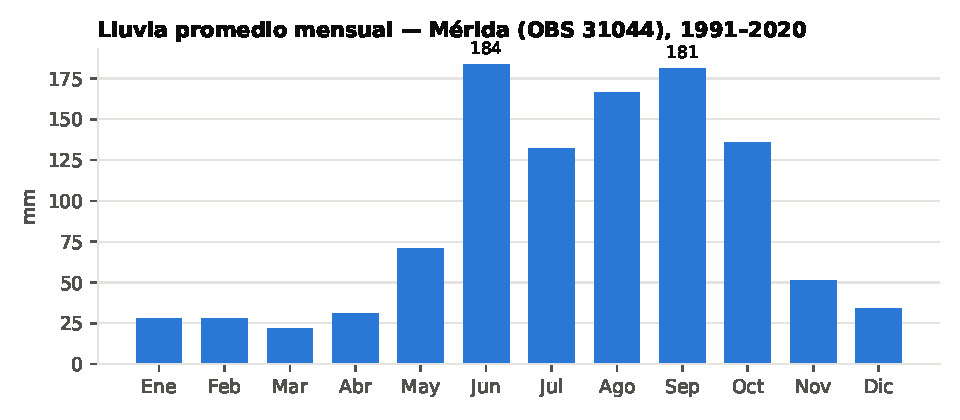
\includegraphics[width=0.9\linewidth]{figuras/v1_climatograma.pdf}\\[6pt]
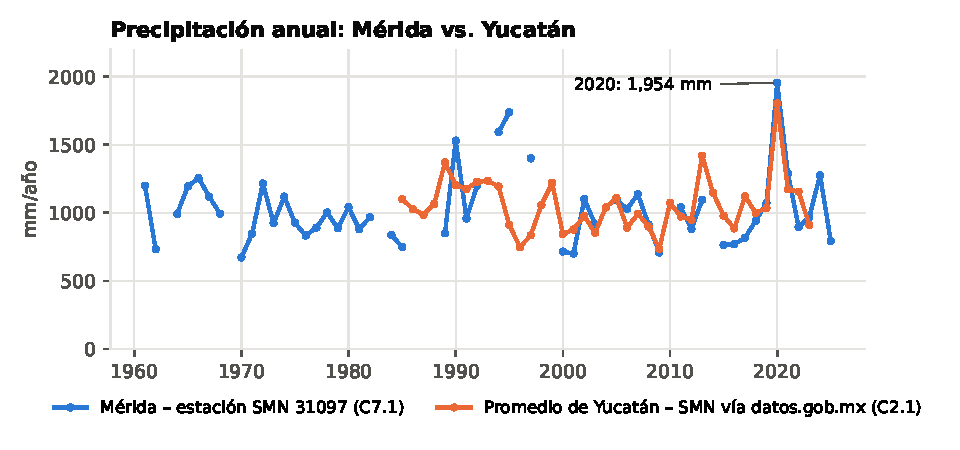
\includegraphics[width=0.9\linewidth]{figuras/v2_serie_anual.pdf}
\end{center}
{\small\color{tinta2} V2: Mérida suele llover más que el promedio de Yucatán, pero sube y baja en los mismos años. Los huecos son años incompletos.}

\begin{center}
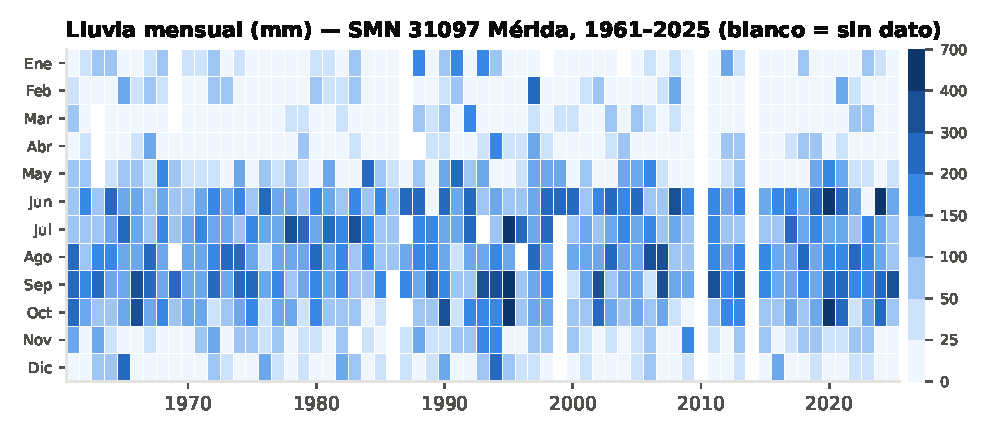
\includegraphics[width=0.93\linewidth]{figuras/v3_heatmap.pdf}\\[6pt]
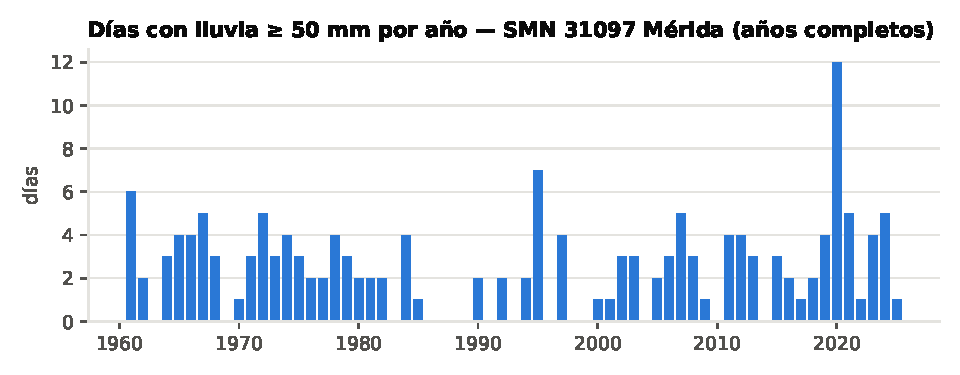
\includegraphics[width=0.9\linewidth]{figuras/v4_dias_intensos.pdf}
\end{center}

\begin{center}
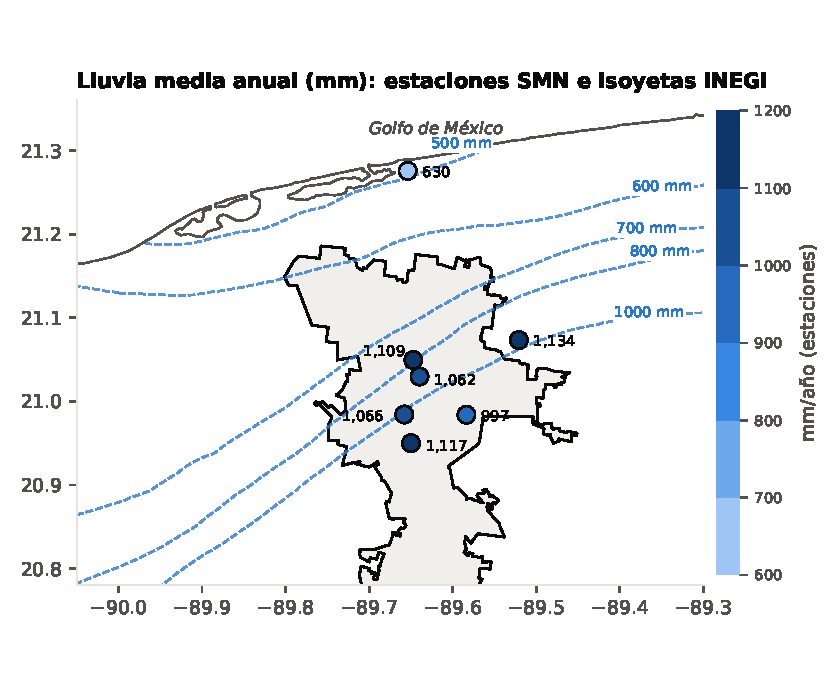
\includegraphics[width=0.78\linewidth]{figuras/v5_mapa.pdf}
\end{center}
{\small\color{tinta2} V5: el área gris es el municipio de Mérida (Marco Geoestadístico INEGI). Las líneas punteadas son las isoyetas de INEGI.
Los círculos son las estaciones del SMN con al menos 10 años completos; el número junto a cada uno es su promedio anual en mm.}

\begin{center}
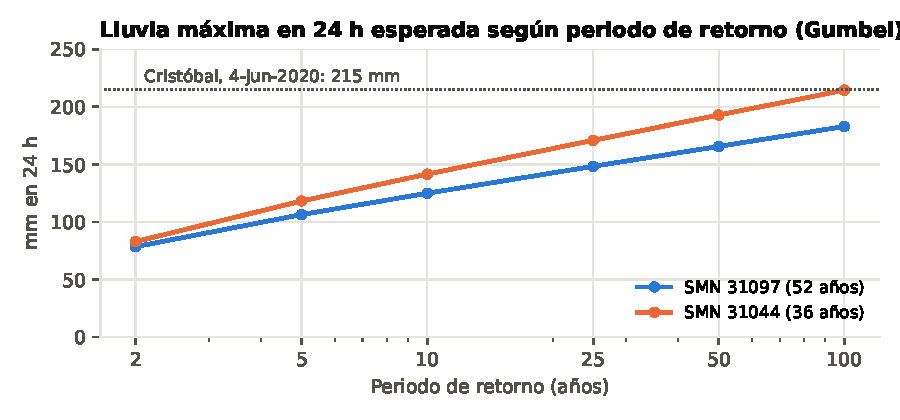
\includegraphics[width=0.85\linewidth]{figuras/v7_periodos_retorno.pdf}
\end{center}

\section{Eventos extraordinarios}

\subsection{Días más lluviosos (estaciones urbanas del SMN)}
{\small
\begin{tabularx}{\linewidth}{@{}llXl@{}}
\toprule
\textbf{Fecha} & \textbf{mm/24 h} & \textbf{Estación} & \textbf{Evento asociado} \\ \midrule
2002-09-23 & 223.0 & C.I.C.Y. (31036) & Huracán Isidoro \\
2020-06-04 & 215.0 & MERIDA (CONAGUA) (31097) & Tormenta tropical Cristóbal \\
1993-06-17 & 169.0 & MERIDA (OBS) (31044) & — \\
2006-09-02 & 167.6 & MERIDA (OBS) (31044) & — \\
2015-08-16 & 164.2 & COLONIA EMILIANO ZAPATA (31095) & — \\
1991-12-04 & 162.0 & MERIDA (OBS) (31044) & — \\
2026-05-30 & 153.6 & MERIDA (OBS) (31044) & — \\
1968-05-23 & 153.5 & MERIDA (CONAGUA) (31097) & — \\
1968-10-23 & 152.5 & MERIDA (CONAGUA) (31097) & — \\
2020-06-02 & 150.3 & COLONIA EMILIANO ZAPATA (31095) & Tormenta tropical Cristóbal \\
2020-10-02 & 150.0 & C.I.C.Y. (31036) & Tormenta tropical Gamma \\
1975-09-15 & 136.0 & MERIDA (CONAGUA) (31097) & — \\
\bottomrule
\end{tabularx}}

\subsection{Declaratorias oficiales por lluvia o ciclón en el municipio de Mérida (CENAPRED, 2000–2023)}
{\small
\begin{tabularx}{\linewidth}{@{}lllX@{}}
\toprule
\textbf{Inicio} & \textbf{Tipo} & \textbf{Fenómeno} & \textbf{Observaciones} \\ \midrule
20/09/2002 & Emergencia & Ciclón Tropical & Huracán Isidore \\
20/09/2002 & Desastre & Lluvias & Lluvias atípicas e impredecibles. Huracán Isidore \\
16/07/2005 & Emergencia & Ciclón Tropical & Huracan "Emily" \\
18/08/2007 & Emergencia & Ciclón Tropical & Huracan Dean \\
01/10/2020 & Emergencia & Lluvias & Lluvia severa e inundación pluvial. Frente Frío No. 4, Tormenta Tropical Gamma y Huracán Delta \\
01/10/2020 & Desastre & Ciclón Tropical & Huracán Delta \\
\bottomrule
\end{tabularx}}

\subsection{Lluvia esperada en 24 h por periodo de retorno (datos propios, C7.2)}
\begin{tabular}{@{}lrr@{}}
\toprule
\textbf{Periodo de retorno (años)} & \textbf{SMN 31097 (mm)} & \textbf{SMN 31044 (mm)} \\ \midrule
2 & 78 & 82 \\
5 & 106 & 116 \\
10 & 124 & 138 \\
25 & 148 & 167 \\
50 & 165 & 188 \\
100 & 182 & 209 \\
\bottomrule
\end{tabular}

\section{Advertencias metodológicas}
\begin{itemize}[leftmargin=1.2em,itemsep=2pt]
\item \textbf{Completitud:} un mes cuenta solo si tiene al menos 80\% de días con dato, y un año solo si tiene los 12 meses válidos.
\item \textbf{Estación ≠ ciudad:} un pluviómetro mide un punto. En una tormenta, dos colonias pueden recibir cantidades muy distintas.
\item \textbf{Intensidad:} los datos diarios no muestran aguaceros cortos (por ejemplo, 60 mm en una hora), que son los que más inundan.
  Para eso sirven C5.1 (solicitud al SMN) y C6.1 (scraping periódico de las estaciones automáticas).
\item \textbf{Periodos de retorno:} son estimaciones con 44–55 años de datos; la incertidumbre crece mucho para 50 y 100 años.
\item \textbf{Elevación:} Mérida es muy plana (0–13 m en el centro); usar el modelo de INEGI con cuidado y validarlo con C8.3.
\end{itemize}

\section{Pendientes}
\begin{enumerate}[leftmargin=1.4em,itemsep=2pt]
\item Enviar las 3 solicitudes de información (C5.1–C5.3); el texto listo para copiar está en \nolinkurl{05_Solicitudes_gobierno/solicitudes_sugeridas.md}.
\item Programar el scraping del SMN (C6.1) para que corra cada semana y vaya acumulando la serie de intensidad.
\item Opcional: crear una cuenta en NASA Earthdata para descargar GEDI/ICESat-2 (C8.3).
\item Conectar \texttt{07\_Datos\_propios/} con el prototipo HTML.
\end{enumerate}

\end{document}
